\documentclass[12pt,oneside]{book}
\usepackage{geometry}                		% See geometry.pdf to learn the layout options. There are lots.
\geometry{a4paper}                   			% ... or a4paper or a5paper or ... 
%\geometry{landscape}                		% Activate for for rotated page geometry
%\usepackage[parfill]{parskip}    		% Activate to begin paragraphs with an empty line rather than an indent
\usepackage{graphicx}				% Use pdf, png, jpg, or epsß with pdflatex; use eps in DVI mode
								% TeX will automatically convert eps --> pdf in pdflatex		
\usepackage{amssymb}

\usepackage[spanish]{babel}			% Permite que partes automáticas del documento aparezcan en castellano.
\usepackage[utf8]{inputenc}			% Permite escribir tildes y otros caracteres directamente en el .tex
\usepackage[T1]{fontenc}				% Asegura que el documento resultante use caracteres de una fuente apropiada.

\usepackage{hyperref}				% Permite poner urls y links dentro del documento

\title{Mi Juego Favorito}
\author{Javier Tibau}
%\date{}							% Activate to display a given date or no date

\begin{document}
\maketitle
\tableofcontents

\chapter{Introducción}
El libro a continuación es creado como una herramienta para el desarrollo de habilidades de edición colaborativa de documentos de texto plano. La herramienta que habilita dicha colaboración, en este taller, es Git pero podría ser reemplazada por otros sistemas de versionamiento.

\chapter{Los Juegos}

\section{Bucaminas}

\begin{figure}[htbp]
\begin{center}
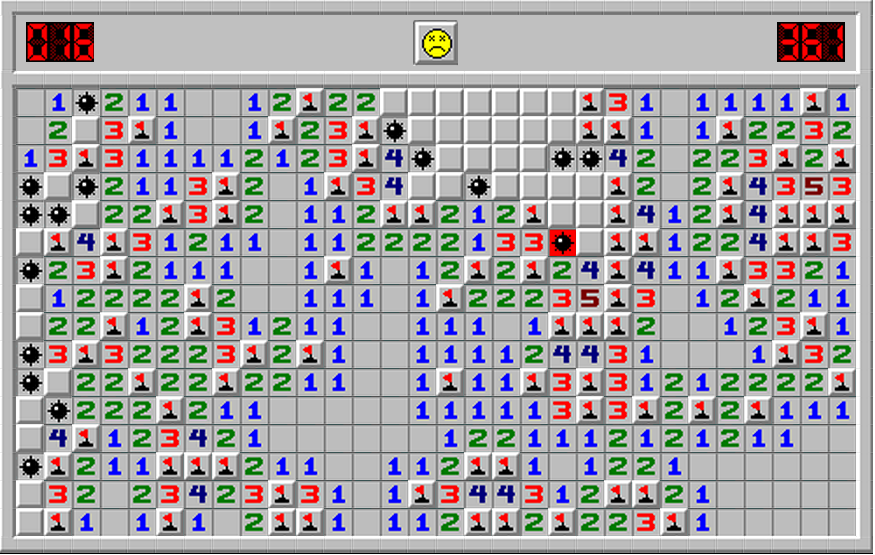
\includegraphics[width=.60\textwidth]{./imagenes/minesweeper.png}
\caption{Buscaminas}
\label{Buscaminas}
\end{center}
\end{figure}
Buscaminas\footnote{\url{http://minesweeperonline.com/}} es uno de los juegos más jugados debido a lo ubicuo de su distribución. Fue incluido en 1992 en la versión de Windows 3.1 y desde entonces lo hemos encontrado presente en todas las versiones de dicho sistema operativo.
En la figura \ref{Buscaminas} puede ver una implementación web del juego.
La premisa del juego es simple: Limpiar el campo de juego sin hacer explotar ninguna de las minas que se encuentran en la cuadrícula.

\subsubsection{¿Por qué es uno de mis juegos favoritos?}
\begin{itemize}
\item[Javier Tibau] Las reglas del juego son sencillas y fáciles de entender. A pesar de esto, el juego no es atractivo para todo el mundo, creo que es un gusto adquirido. Las reglas me fueron presentadas por mi papá, quien en su máquina de trabajo con Windows 3.11 era uno de los pocos juegos ``divertidos'' que tenía. Para mi, el gran interés del juego es que destaca (o esconde) la resolución de problemas con fondo algebraico. En cierto momento del juego, y para el jugador que ha estudiado álgebra lineal, el reventar una casilla se torna similar a descifrar un sistema de ecuaciones con varias incógnitas. Los sistemas sencillos son bien definidos y tienen 2, 3 o hasta 4 incógnitas, mientras los más complejos pueden inclusive tener múltiples soluciones.
\end{itemize}

\section{Dota 2}

\begin{figure}[htbp]
\begin{center}
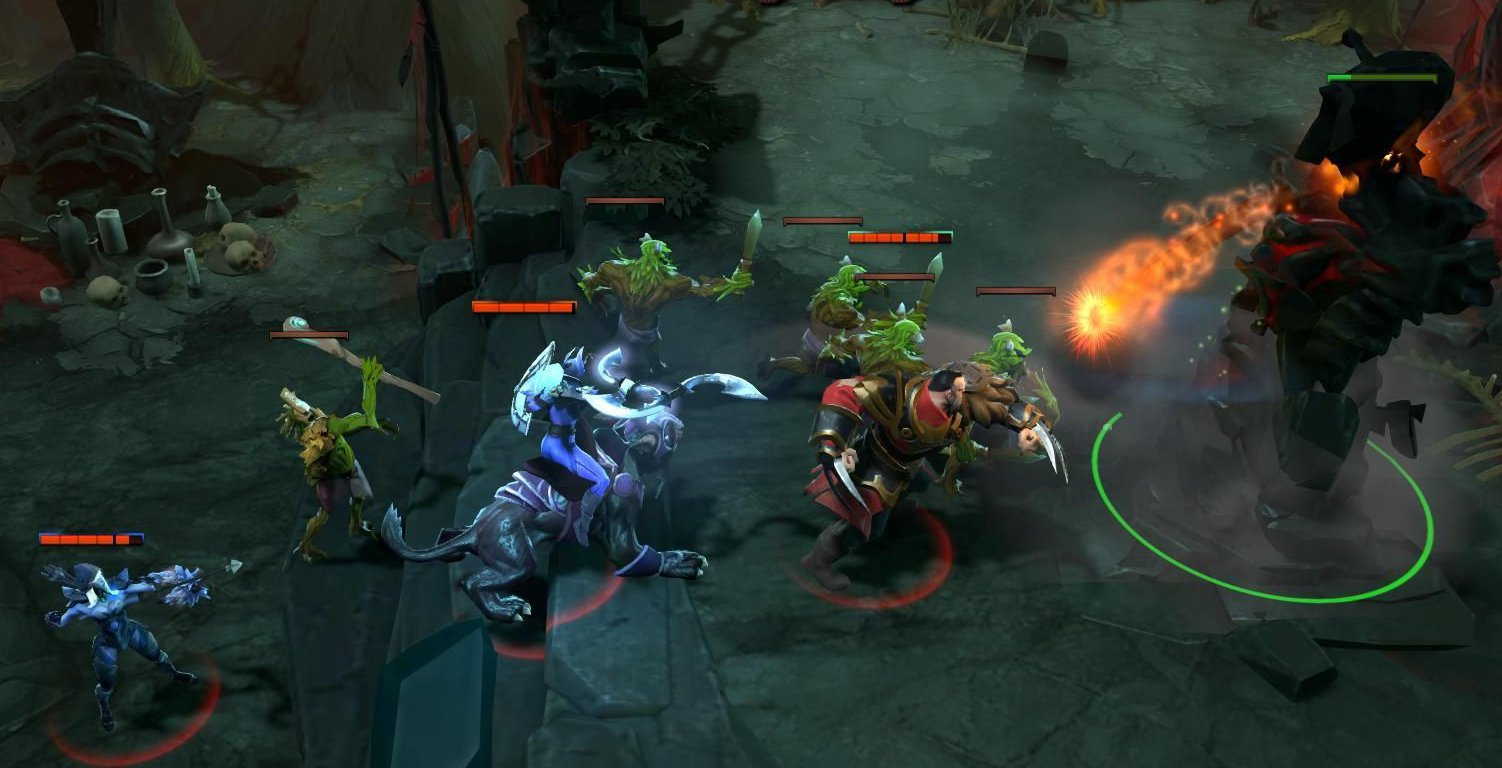
\includegraphics[width=.60\textwidth]{./imagenes/dota2.jpg}
\caption{Dota 2}
\label{Dota 2}
\end{center}
\end{figure}
Dota 2 \footnote{\url{http://dota2.com/}} es un juego creado por Valve basado en el popular mod de Warcraft 3, Defense of the Ancients. Es un juego de estrategia en equipo para ser jugado con equipos de 5 personas cada uno.
Dota 2 combina elementos de estrategia en tiempo real con perspectiva "en tercera persona", incorporando a todo ello un sistema de nivelación y jugabilidad de diversos juegos de rol como Diablo. Los jugadores asumen el papel de una unidad clasificado como un "héroe", que puede subir de nivel hasta un máximo de 25. La configuración básica de Dota 2 consiste en dos ciudades de distinta forma, cada una cuenta con una fortaleza de defensa conocida como "ancestro", situadas en los extremos opuestos de un mapa equilibrado de manera uniforme. Entre ellas hay varias regiones de conexión identificado como "caminos", que son atravesados por unidades enemigas, al tiempo que luchan contra poderosas torres defensivas a lo largo del camino. Los jugadores se dividen entre dos equipos, cada uno con hasta cinco jugadores, para competir como los principales defensores de cada Fortaleza de los Ancestros.

\subsubsection{¿Por qué es uno de mis juegos favoritos?}
\begin{itemize}
\item[Victor Cedeño] Este es un juego que requiere de comunicación y cooperación entre 5 personas para poder lograr el objetivo de vencer al otro equipo. Es muy dificil jugar solo sin la ayuda de tus compañeros. El juego tiene una gran selección de mas de 100 heroes para elegir, esto quiere decir que cada partida es diferente ya que las combinaciones posibles de los equipos son innumerables. Es un juego que fomenta el trabajo en equipo y las decisiones correctas.
\end{itemize}
\section{Zelda: Skyward Sword}

\begin{figure}[htbp]
\begin{center}
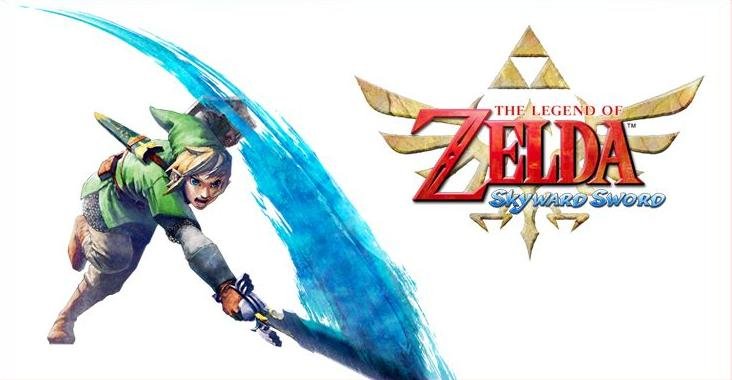
\includegraphics[width=.60\textwidth]{./imagenes/skyward.jpg}
\caption{Zelda: Skyward Sword}
\label{Zelda: Skyward Sword}
\end{center}
\end{figure}
Zelda: Skyward Sword\footnote{\url{http://zelda.com/skywardsword/}} es el primer Zelda en ofrecerte total control de la espada y escudo via wiimote + nunchuck. Fue publicado en Noviembre del 2011 y ha sido uno de los juegos de Zelda más controversiales por su único modo de jugarlo con controles de movimiento.

La premisa del juego es que eres un chico (Link) que vive en una comunidad en una isla flotante y debes emprender un viaje a la superficie (Hyrule) para rescatar a Zelda.

\subsubsection{¿Por qué es uno de mis juegos favoritos?}
\begin{itemize}
\item[Gianni Carlo] Las reglas del juego son similares a los anteriores juegos de Zelda con el agregado que ahora cada enemigo fue diseñado con los controles de moviemiento en mente, no basta con agitar de izquierda a derecha el control para poder pasar el juego, y esto ayuda en gran parte a sumergirte en el juego ya que debes atacar de cierta forma a los enemigos y/o repeler ataques con tu escudo en el momento preciso sino recibes una penalidad. A pesar de esto, el juego no es atractivo para todo el mundo debido a la única opción de controles a los que alegan que no responden con suficiente precisión o a veces ni responden. Para mi, el gran interés del juego, aparte de presentar el origen de la historia del universo de Zelda, es el nuevo estilo de jugarlo y la experiencia de inmersión única que presenta a cualquier fan de la serie (los motion controls de Twilight Princess para Wii no cuentan en mi opinión ya que eran tan solo un test para ver que tan buena sería la acogida para implementarlo como única opción en el siguiente Zelda).
\end{itemize}
\section{Counter-Strike}

\begin{figure}[htbp]
\begin{center}
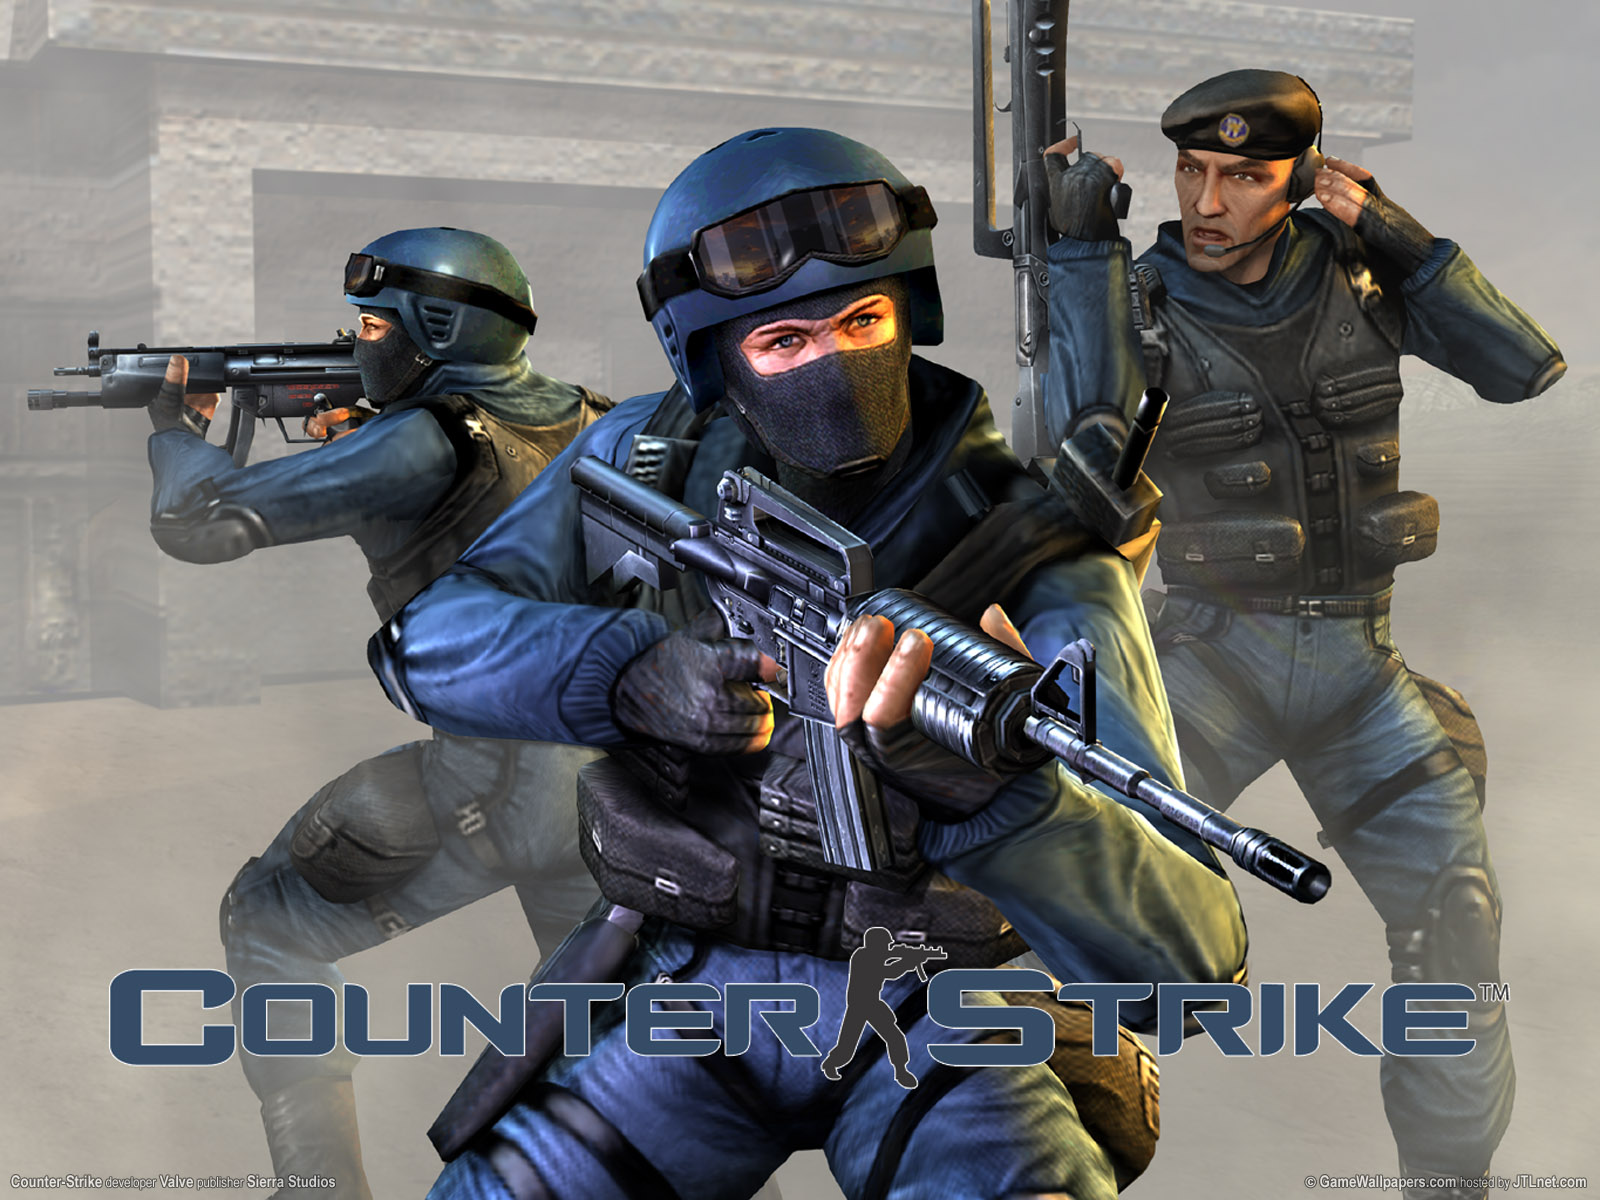
\includegraphics[width=.60\textwidth]{./imagenes/CounterStrike.jpg}
\caption{Counter-Strike}
\label{Counter-Strike}
\end{center}
\end{figure}
Counter-Strike\footnote{\url{http://http://store.steampowered.com/css/}} es un juego de tipo multijugador. La acción de Counter-Strike se desarrolla en rondas de una duración elegida por el que las crea, en la cual un equipo de terroristas se enfrenta a un equipo de antiterrorista. El equipo victorioso es el que cumpla todos sus objetivos de victoria, de situación o la eliminación de todos los jugadores del otro equipo. Si al final de la ronda no hay victoria directa de uno de los dos equipos, el equipo que no realizó sus objetivos pierde por eliminación.

\subsubsection{¿Por qué es uno de mis juegos favoritos?}
\begin{itemize}
\item[Edwin Hermenejildo] Counter-Strike Agrupa varios aspectos del espíritu deportista: trabajo de equipo, competencia, igualdad de oportunidades y con su éxito es lógico que el juego haya dado a un gran número de jugadores el deseo de competir.
Todos los jugadores comienzan con la misma cantidad de puntos de vida y la cantidad de puntos de armadura que consiguieron conservar durante la ronda anterior siempre y cuando no compren una nueva. Cuando los daños son causados por los disparos de sus adversarios o sus compañeros -si hay fuego amigo- (los compañeros causan menos daño, pero pueden matar igualmente), así como por una caída violenta los puntos de vida del jugador disminuyen. Los disparos se pueden localizar en diferentes partes del cuerpo (brazo derecho e izquierdo, pierna derecha e izquierda, torso, y cabeza), y causan más o menos daños según el lugar afectado, sabiendo que un disparo en la cabeza o headshot es a menudo mortal. La pérdida de puntos de vida solo causa una pequeña disminución en los movimientos del terrorista o antiterrorista que haya recibido el daño. Cuando la totalidad de los puntos de vida se terminan, el jugador muere.
\end{itemize}



\chapter{Conclusiones}
Cuales juegos fueron más populares y un breve razonamiento del porqué.

\end{document}  
